\documentclass[tikz,border=5]{standalone}
\usepackage{amssymb,enumerate,psfrag,graphicx,amsfonts,amsrefs,amsthm,mathrsfs,amsmath,amscd,version,graphicx}
\usepackage{xcolor}
\usepackage{tikz-cd}
\usepackage{tikz}
\usetikzlibrary{arrows}
\tikzset{
    vertex/.style={draw,circle,inner sep=2 pt, minimum size=6pt},
    edge/.style={thick},
    dedge/.style ={->,> = latex',thick}
    }
\usetikzlibrary{decorations.markings}
\usetikzlibrary{arrows.meta}

\begin{document}

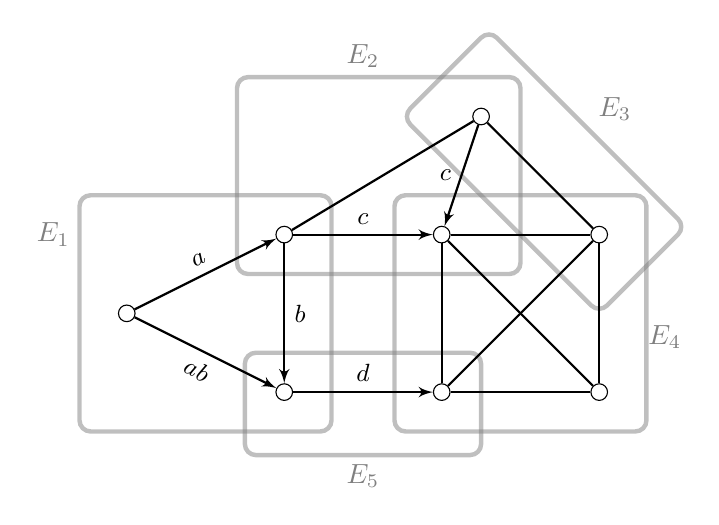
\begin{tikzpicture}
\draw[ultra thick, gray,opacity=0.5, rounded corners] (-0.6,-1.5) rectangle (2.6,1.5);
\node[gray,left] at (-0.6,1){$E_1$};


\draw[ultra thick, gray,opacity=0.5,rounded corners] (1.4,0.5) rectangle (5,3);
\node[gray,above] at (3,3){$E_2$};

\draw[ultra thick, gray,opacity=0.5,rounded corners] (1.5,-0.5) rectangle (4.5,-1.8);
\node[gray,below] at (3,-1.8){$E_5$};

\draw[ultra thick, gray,opacity=0.5,rounded corners] (3.4,-1.5) rectangle (6.6,1.5);
\node[gray,right] at (6.5,-0.3){$E_4$};


\draw[ultra thick, gray,opacity=0.5,rounded corners] (3.5,2.5)--(4.6,3.6)--(7.1,1.1)--(6,0)--cycle;
\node[gray] at (6.2,2.6){$E_3$};
% vertices
\node[vertex]  (1) at (0,0){};
\node[vertex]  (2) at (2,1) {};
\node[vertex]  (3) at (2,-1) {};

\node[vertex]  (4) at (4,-1) {};
\node[vertex]  (5) at (4,1) {};
\node[vertex]  (6) at (6,-1) {};
\node[vertex]  (7) at (6,1) {};
\node[vertex]  (8) at (4.5,2.5) {};




%edges
\draw[dedge] (1) -- (2) node[midway, above,sloped] {\small $a$};
\draw[dedge] (2) -- (3) node[midway, right] {\small $b$};
\draw[dedge] (1) -- (3) node[midway, below,sloped] {\small $ab$};

\draw[dedge] (2) -- (5) node[midway, above,sloped] {\small $c$};
\draw[dedge] (8) -- (5) node[midway,left] {\small $c$};
\draw[edge] (2) -- (8) node[midway, above,sloped] {\tiny };

\draw[edge] (8) -- (7) node[midway, above,sloped] {\tiny };

\draw[dedge] (3) -- (4) node[midway, above,sloped] {\small $d$};

\draw[edge] (4) -- (5) node[midway, left] {\tiny };
\draw[edge] (4) -- (6) node[midway, below,sloped] {\tiny };
\draw[edge] (4) -- (7) node[pos=0.35, above,sloped] {\tiny };
\draw[edge] (5) -- (6) node[pos=0.65, above,sloped] {\tiny };
\draw[edge] (5) -- (7) node[pos=0.67, above,sloped] {\tiny };
\draw[edge] (6) -- (7) node[midway, right] {\tiny };



\end{tikzpicture}

\end{document}